% Created by tikzDevice version 0.12 on 2019-04-06 22:04:40
% !TEX encoding = UTF-8 Unicode
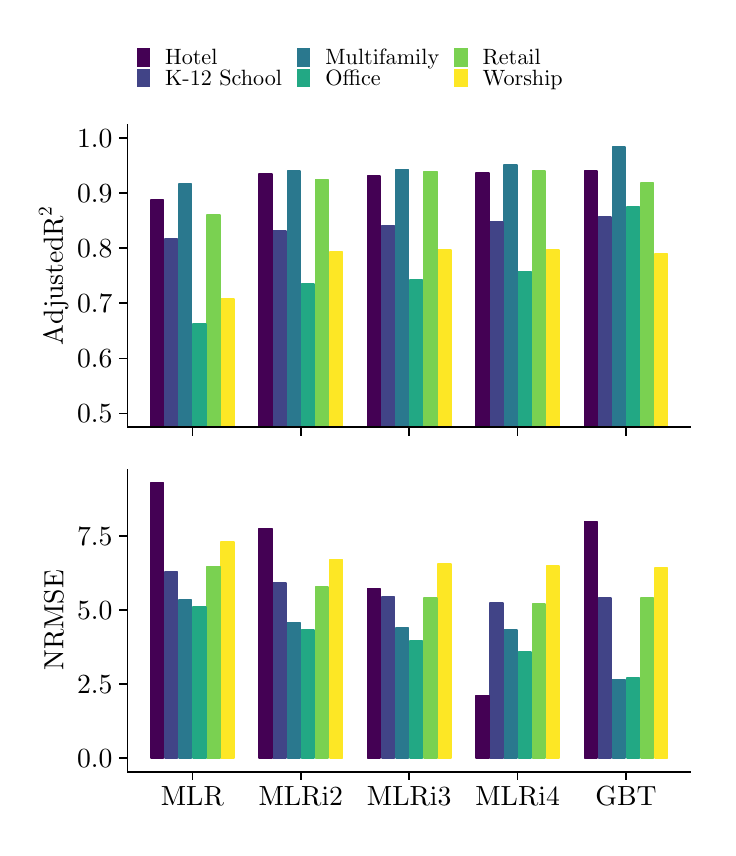
\begin{tikzpicture}[x=1pt,y=1pt]
\definecolor{fillColor}{RGB}{255,255,255}
\path[use as bounding box,fill=fillColor,fill opacity=0.00] (0,0) rectangle (245.72,289.08);
\begin{scope}
\path[clip] (  0.00,135.70) rectangle (245.72,289.08);
\definecolor{drawColor}{RGB}{255,255,255}
\definecolor{fillColor}{RGB}{255,255,255}

\path[draw=drawColor,line width= 0.6pt,line join=round,line cap=round,fill=fillColor] (  0.00,135.70) rectangle (245.72,289.08);
\end{scope}
\begin{scope}
\path[clip] (  0.00,  0.00) rectangle (245.72,135.70);
\definecolor{drawColor}{RGB}{255,255,255}
\definecolor{fillColor}{RGB}{255,255,255}

\path[draw=drawColor,line width= 0.6pt,line join=round,line cap=round,fill=fillColor] (  0.00,  0.00) rectangle (245.72,135.70);
\end{scope}
\begin{scope}
\path[clip] ( 36.01,144.70) rectangle (239.72,254.17);
\definecolor{fillColor}{RGB}{255,255,255}

\path[fill=fillColor] ( 36.01,144.70) rectangle (239.72,254.17);
\definecolor{drawColor}{RGB}{253,231,37}
\definecolor{fillColor}{RGB}{253,231,37}

\path[draw=drawColor,line width= 0.6pt,line join=round,fill=fillColor] ( 69.96, 50.16) rectangle ( 74.53,191.08);
\definecolor{drawColor}{RGB}{122,209,81}
\definecolor{fillColor}{RGB}{122,209,81}

\path[draw=drawColor,line width= 0.6pt,line join=round,fill=fillColor] ( 64.87, 50.16) rectangle ( 69.44,221.33);
\definecolor{drawColor}{RGB}{34,168,132}
\definecolor{fillColor}{RGB}{34,168,132}

\path[draw=drawColor,line width= 0.6pt,line join=round,fill=fillColor] ( 59.77, 50.16) rectangle ( 64.34,181.92);
\definecolor{drawColor}{RGB}{42,120,142}
\definecolor{fillColor}{RGB}{42,120,142}

\path[draw=drawColor,line width= 0.6pt,line join=round,fill=fillColor] ( 54.68, 50.16) rectangle ( 59.25,232.68);
\definecolor{drawColor}{RGB}{65,68,135}
\definecolor{fillColor}{RGB}{65,68,135}

\path[draw=drawColor,line width= 0.6pt,line join=round,fill=fillColor] ( 49.59, 50.16) rectangle ( 54.16,212.77);
\definecolor{drawColor}{RGB}{68,1,84}
\definecolor{fillColor}{RGB}{68,1,84}

\path[draw=drawColor,line width= 0.6pt,line join=round,fill=fillColor] ( 44.49, 50.16) rectangle ( 49.06,226.90);
\definecolor{drawColor}{RGB}{253,231,37}
\definecolor{fillColor}{RGB}{253,231,37}

\path[draw=drawColor,line width= 0.6pt,line join=round,fill=fillColor] (109.13, 50.16) rectangle (113.70,208.00);
\definecolor{drawColor}{RGB}{122,209,81}
\definecolor{fillColor}{RGB}{122,209,81}

\path[draw=drawColor,line width= 0.6pt,line join=round,fill=fillColor] (104.04, 50.16) rectangle (108.61,234.27);
\definecolor{drawColor}{RGB}{34,168,132}
\definecolor{fillColor}{RGB}{34,168,132}

\path[draw=drawColor,line width= 0.6pt,line join=round,fill=fillColor] ( 98.95, 50.16) rectangle (103.52,196.45);
\definecolor{drawColor}{RGB}{42,120,142}
\definecolor{fillColor}{RGB}{42,120,142}

\path[draw=drawColor,line width= 0.6pt,line join=round,fill=fillColor] ( 93.85, 50.16) rectangle ( 98.43,237.25);
\definecolor{drawColor}{RGB}{65,68,135}
\definecolor{fillColor}{RGB}{65,68,135}

\path[draw=drawColor,line width= 0.6pt,line join=round,fill=fillColor] ( 88.76, 50.16) rectangle ( 93.33,215.56);
\definecolor{drawColor}{RGB}{68,1,84}
\definecolor{fillColor}{RGB}{68,1,84}

\path[draw=drawColor,line width= 0.6pt,line join=round,fill=fillColor] ( 83.67, 50.16) rectangle ( 88.24,236.26);
\definecolor{drawColor}{RGB}{253,231,37}
\definecolor{fillColor}{RGB}{253,231,37}

\path[draw=drawColor,line width= 0.6pt,line join=round,fill=fillColor] (148.31, 50.16) rectangle (152.88,208.79);
\definecolor{drawColor}{RGB}{122,209,81}
\definecolor{fillColor}{RGB}{122,209,81}

\path[draw=drawColor,line width= 0.6pt,line join=round,fill=fillColor] (143.22, 50.16) rectangle (147.79,237.06);
\definecolor{drawColor}{RGB}{34,168,132}
\definecolor{fillColor}{RGB}{34,168,132}

\path[draw=drawColor,line width= 0.6pt,line join=round,fill=fillColor] (138.12, 50.16) rectangle (142.69,197.84);
\definecolor{drawColor}{RGB}{42,120,142}
\definecolor{fillColor}{RGB}{42,120,142}

\path[draw=drawColor,line width= 0.6pt,line join=round,fill=fillColor] (133.03, 50.16) rectangle (137.60,237.85);
\definecolor{drawColor}{RGB}{65,68,135}
\definecolor{fillColor}{RGB}{65,68,135}

\path[draw=drawColor,line width= 0.6pt,line join=round,fill=fillColor] (127.94, 50.16) rectangle (132.51,217.55);
\definecolor{drawColor}{RGB}{68,1,84}
\definecolor{fillColor}{RGB}{68,1,84}

\path[draw=drawColor,line width= 0.6pt,line join=round,fill=fillColor] (122.84, 50.16) rectangle (127.42,235.46);
\definecolor{drawColor}{RGB}{253,231,37}
\definecolor{fillColor}{RGB}{253,231,37}

\path[draw=drawColor,line width= 0.6pt,line join=round,fill=fillColor] (187.48, 50.16) rectangle (192.05,208.79);
\definecolor{drawColor}{RGB}{122,209,81}
\definecolor{fillColor}{RGB}{122,209,81}

\path[draw=drawColor,line width= 0.6pt,line join=round,fill=fillColor] (182.39, 50.16) rectangle (186.96,237.25);
\definecolor{drawColor}{RGB}{34,168,132}
\definecolor{fillColor}{RGB}{34,168,132}

\path[draw=drawColor,line width= 0.6pt,line join=round,fill=fillColor] (177.30, 50.16) rectangle (181.87,201.03);
\definecolor{drawColor}{RGB}{42,120,142}
\definecolor{fillColor}{RGB}{42,120,142}

\path[draw=drawColor,line width= 0.6pt,line join=round,fill=fillColor] (172.21, 50.16) rectangle (176.78,239.44);
\definecolor{drawColor}{RGB}{65,68,135}
\definecolor{fillColor}{RGB}{65,68,135}

\path[draw=drawColor,line width= 0.6pt,line join=round,fill=fillColor] (167.11, 50.16) rectangle (171.68,218.74);
\definecolor{drawColor}{RGB}{68,1,84}
\definecolor{fillColor}{RGB}{68,1,84}

\path[draw=drawColor,line width= 0.6pt,line join=round,fill=fillColor] (162.02, 50.16) rectangle (166.59,236.66);
\definecolor{drawColor}{RGB}{253,231,37}
\definecolor{fillColor}{RGB}{253,231,37}

\path[draw=drawColor,line width= 0.6pt,line join=round,fill=fillColor] (226.66, 50.16) rectangle (231.23,207.40);
\definecolor{drawColor}{RGB}{122,209,81}
\definecolor{fillColor}{RGB}{122,209,81}

\path[draw=drawColor,line width= 0.6pt,line join=round,fill=fillColor] (221.57, 50.16) rectangle (226.14,232.88);
\definecolor{drawColor}{RGB}{34,168,132}
\definecolor{fillColor}{RGB}{34,168,132}

\path[draw=drawColor,line width= 0.6pt,line join=round,fill=fillColor] (216.47, 50.16) rectangle (221.04,224.32);
\definecolor{drawColor}{RGB}{42,120,142}
\definecolor{fillColor}{RGB}{42,120,142}

\path[draw=drawColor,line width= 0.6pt,line join=round,fill=fillColor] (211.38, 50.16) rectangle (215.95,246.01);
\definecolor{drawColor}{RGB}{65,68,135}
\definecolor{fillColor}{RGB}{65,68,135}

\path[draw=drawColor,line width= 0.6pt,line join=round,fill=fillColor] (206.29, 50.16) rectangle (210.86,220.73);
\definecolor{drawColor}{RGB}{68,1,84}
\definecolor{fillColor}{RGB}{68,1,84}

\path[draw=drawColor,line width= 0.6pt,line join=round,fill=fillColor] (201.20, 50.16) rectangle (205.77,237.25);
\end{scope}
\begin{scope}
\path[clip] ( 36.01, 20.23) rectangle (239.72,129.70);
\definecolor{fillColor}{RGB}{255,255,255}

\path[fill=fillColor] ( 36.01, 20.23) rectangle (239.72,129.70);
\definecolor{drawColor}{RGB}{253,231,37}
\definecolor{fillColor}{RGB}{253,231,37}

\path[draw=drawColor,line width= 0.6pt,line join=round,fill=fillColor] ( 69.96, 25.21) rectangle ( 74.53,103.20);
\definecolor{drawColor}{RGB}{122,209,81}
\definecolor{fillColor}{RGB}{122,209,81}

\path[draw=drawColor,line width= 0.6pt,line join=round,fill=fillColor] ( 64.87, 25.21) rectangle ( 69.44, 94.43);
\definecolor{drawColor}{RGB}{34,168,132}
\definecolor{fillColor}{RGB}{34,168,132}

\path[draw=drawColor,line width= 0.6pt,line join=round,fill=fillColor] ( 59.77, 25.21) rectangle ( 64.34, 79.69);
\definecolor{drawColor}{RGB}{42,120,142}
\definecolor{fillColor}{RGB}{42,120,142}

\path[draw=drawColor,line width= 0.6pt,line join=round,fill=fillColor] ( 54.68, 25.21) rectangle ( 59.25, 82.37);
\definecolor{drawColor}{RGB}{65,68,135}
\definecolor{fillColor}{RGB}{65,68,135}

\path[draw=drawColor,line width= 0.6pt,line join=round,fill=fillColor] ( 49.59, 25.21) rectangle ( 54.16, 92.38);
\definecolor{drawColor}{RGB}{68,1,84}
\definecolor{fillColor}{RGB}{68,1,84}

\path[draw=drawColor,line width= 0.6pt,line join=round,fill=fillColor] ( 44.49, 25.21) rectangle ( 49.06,124.73);
\definecolor{drawColor}{RGB}{253,231,37}
\definecolor{fillColor}{RGB}{253,231,37}

\path[draw=drawColor,line width= 0.6pt,line join=round,fill=fillColor] (109.13, 25.21) rectangle (113.70, 96.96);
\definecolor{drawColor}{RGB}{122,209,81}
\definecolor{fillColor}{RGB}{122,209,81}

\path[draw=drawColor,line width= 0.6pt,line join=round,fill=fillColor] (104.04, 25.21) rectangle (108.61, 86.88);
\definecolor{drawColor}{RGB}{34,168,132}
\definecolor{fillColor}{RGB}{34,168,132}

\path[draw=drawColor,line width= 0.6pt,line join=round,fill=fillColor] ( 98.95, 25.21) rectangle (103.52, 71.44);
\definecolor{drawColor}{RGB}{42,120,142}
\definecolor{fillColor}{RGB}{42,120,142}

\path[draw=drawColor,line width= 0.6pt,line join=round,fill=fillColor] ( 93.85, 25.21) rectangle ( 98.43, 74.16);
\definecolor{drawColor}{RGB}{65,68,135}
\definecolor{fillColor}{RGB}{65,68,135}

\path[draw=drawColor,line width= 0.6pt,line join=round,fill=fillColor] ( 88.76, 25.21) rectangle ( 93.33, 88.48);
\definecolor{drawColor}{RGB}{68,1,84}
\definecolor{fillColor}{RGB}{68,1,84}

\path[draw=drawColor,line width= 0.6pt,line join=round,fill=fillColor] ( 83.67, 25.21) rectangle ( 88.24,108.12);
\definecolor{drawColor}{RGB}{253,231,37}
\definecolor{fillColor}{RGB}{253,231,37}

\path[draw=drawColor,line width= 0.6pt,line join=round,fill=fillColor] (148.31, 25.21) rectangle (152.88, 95.22);
\definecolor{drawColor}{RGB}{122,209,81}
\definecolor{fillColor}{RGB}{122,209,81}

\path[draw=drawColor,line width= 0.6pt,line join=round,fill=fillColor] (143.22, 25.21) rectangle (147.79, 83.10);
\definecolor{drawColor}{RGB}{34,168,132}
\definecolor{fillColor}{RGB}{34,168,132}

\path[draw=drawColor,line width= 0.6pt,line join=round,fill=fillColor] (138.12, 25.21) rectangle (142.69, 67.57);
\definecolor{drawColor}{RGB}{42,120,142}
\definecolor{fillColor}{RGB}{42,120,142}

\path[draw=drawColor,line width= 0.6pt,line join=round,fill=fillColor] (133.03, 25.21) rectangle (137.60, 72.24);
\definecolor{drawColor}{RGB}{65,68,135}
\definecolor{fillColor}{RGB}{65,68,135}

\path[draw=drawColor,line width= 0.6pt,line join=round,fill=fillColor] (127.94, 25.21) rectangle (132.51, 83.26);
\definecolor{drawColor}{RGB}{68,1,84}
\definecolor{fillColor}{RGB}{68,1,84}

\path[draw=drawColor,line width= 0.6pt,line join=round,fill=fillColor] (122.84, 25.21) rectangle (127.42, 86.48);
\definecolor{drawColor}{RGB}{253,231,37}
\definecolor{fillColor}{RGB}{253,231,37}

\path[draw=drawColor,line width= 0.6pt,line join=round,fill=fillColor] (187.48, 25.21) rectangle (192.05, 94.55);
\definecolor{drawColor}{RGB}{122,209,81}
\definecolor{fillColor}{RGB}{122,209,81}

\path[draw=drawColor,line width= 0.6pt,line join=round,fill=fillColor] (182.39, 25.21) rectangle (186.96, 80.88);
\definecolor{drawColor}{RGB}{34,168,132}
\definecolor{fillColor}{RGB}{34,168,132}

\path[draw=drawColor,line width= 0.6pt,line join=round,fill=fillColor] (177.30, 25.21) rectangle (181.87, 63.56);
\definecolor{drawColor}{RGB}{42,120,142}
\definecolor{fillColor}{RGB}{42,120,142}

\path[draw=drawColor,line width= 0.6pt,line join=round,fill=fillColor] (172.21, 25.21) rectangle (176.78, 71.41);
\definecolor{drawColor}{RGB}{65,68,135}
\definecolor{fillColor}{RGB}{65,68,135}

\path[draw=drawColor,line width= 0.6pt,line join=round,fill=fillColor] (167.11, 25.21) rectangle (171.68, 81.27);
\definecolor{drawColor}{RGB}{68,1,84}
\definecolor{fillColor}{RGB}{68,1,84}

\path[draw=drawColor,line width= 0.6pt,line join=round,fill=fillColor] (162.02, 25.21) rectangle (166.59, 47.77);
\definecolor{drawColor}{RGB}{253,231,37}
\definecolor{fillColor}{RGB}{253,231,37}

\path[draw=drawColor,line width= 0.6pt,line join=round,fill=fillColor] (226.66, 25.21) rectangle (231.23, 93.86);
\definecolor{drawColor}{RGB}{122,209,81}
\definecolor{fillColor}{RGB}{122,209,81}

\path[draw=drawColor,line width= 0.6pt,line join=round,fill=fillColor] (221.57, 25.21) rectangle (226.14, 83.03);
\definecolor{drawColor}{RGB}{34,168,132}
\definecolor{fillColor}{RGB}{34,168,132}

\path[draw=drawColor,line width= 0.6pt,line join=round,fill=fillColor] (216.47, 25.21) rectangle (221.04, 54.02);
\definecolor{drawColor}{RGB}{42,120,142}
\definecolor{fillColor}{RGB}{42,120,142}

\path[draw=drawColor,line width= 0.6pt,line join=round,fill=fillColor] (211.38, 25.21) rectangle (215.95, 53.58);
\definecolor{drawColor}{RGB}{65,68,135}
\definecolor{fillColor}{RGB}{65,68,135}

\path[draw=drawColor,line width= 0.6pt,line join=round,fill=fillColor] (206.29, 25.21) rectangle (210.86, 83.03);
\definecolor{drawColor}{RGB}{68,1,84}
\definecolor{fillColor}{RGB}{68,1,84}

\path[draw=drawColor,line width= 0.6pt,line join=round,fill=fillColor] (201.20, 25.21) rectangle (205.77,110.63);
\end{scope}
\begin{scope}
\path[clip] (  0.00,  0.00) rectangle (245.72,289.08);
\definecolor{drawColor}{RGB}{0,0,0}

\path[draw=drawColor,line width= 0.6pt,line join=round] ( 36.01,144.70) --
	( 36.01,254.17);
\end{scope}
\begin{scope}
\path[clip] (  0.00,  0.00) rectangle (245.72,289.08);
\definecolor{drawColor}{RGB}{0,0,0}

\node[text=drawColor,anchor=base east,inner sep=0pt, outer sep=0pt, scale=  1.00] at ( 30.61,146.23) {0.5};

\node[text=drawColor,anchor=base east,inner sep=0pt, outer sep=0pt, scale=  1.00] at ( 30.61,166.14) {0.6};

\node[text=drawColor,anchor=base east,inner sep=0pt, outer sep=0pt, scale=  1.00] at ( 30.61,186.04) {0.7};

\node[text=drawColor,anchor=base east,inner sep=0pt, outer sep=0pt, scale=  1.00] at ( 30.61,205.95) {0.8};

\node[text=drawColor,anchor=base east,inner sep=0pt, outer sep=0pt, scale=  1.00] at ( 30.61,225.85) {0.9};

\node[text=drawColor,anchor=base east,inner sep=0pt, outer sep=0pt, scale=  1.00] at ( 30.61,245.75) {1.0};
\end{scope}
\begin{scope}
\path[clip] (  0.00,  0.00) rectangle (245.72,289.08);
\definecolor{drawColor}{RGB}{0,0,0}

\path[draw=drawColor,line width= 0.6pt,line join=round] ( 33.01,149.68) --
	( 36.01,149.68);

\path[draw=drawColor,line width= 0.6pt,line join=round] ( 33.01,169.58) --
	( 36.01,169.58);

\path[draw=drawColor,line width= 0.6pt,line join=round] ( 33.01,189.49) --
	( 36.01,189.49);

\path[draw=drawColor,line width= 0.6pt,line join=round] ( 33.01,209.39) --
	( 36.01,209.39);

\path[draw=drawColor,line width= 0.6pt,line join=round] ( 33.01,229.29) --
	( 36.01,229.29);

\path[draw=drawColor,line width= 0.6pt,line join=round] ( 33.01,249.20) --
	( 36.01,249.20);
\end{scope}
\begin{scope}
\path[clip] (  0.00,  0.00) rectangle (245.72,289.08);
\definecolor{drawColor}{RGB}{0,0,0}

\path[draw=drawColor,line width= 0.6pt,line join=round] ( 36.01, 20.23) --
	( 36.01,129.70);
\end{scope}
\begin{scope}
\path[clip] (  0.00,  0.00) rectangle (245.72,289.08);
\definecolor{drawColor}{RGB}{0,0,0}

\node[text=drawColor,anchor=base east,inner sep=0pt, outer sep=0pt, scale=  1.00] at ( 30.61, 21.76) {0.0};

\node[text=drawColor,anchor=base east,inner sep=0pt, outer sep=0pt, scale=  1.00] at ( 30.61, 48.46) {2.5};

\node[text=drawColor,anchor=base east,inner sep=0pt, outer sep=0pt, scale=  1.00] at ( 30.61, 75.16) {5.0};

\node[text=drawColor,anchor=base east,inner sep=0pt, outer sep=0pt, scale=  1.00] at ( 30.61,101.86) {7.5};
\end{scope}
\begin{scope}
\path[clip] (  0.00,  0.00) rectangle (245.72,289.08);
\definecolor{drawColor}{RGB}{0,0,0}

\path[draw=drawColor,line width= 0.6pt,line join=round] ( 33.01, 25.21) --
	( 36.01, 25.21);

\path[draw=drawColor,line width= 0.6pt,line join=round] ( 33.01, 51.90) --
	( 36.01, 51.90);

\path[draw=drawColor,line width= 0.6pt,line join=round] ( 33.01, 78.60) --
	( 36.01, 78.60);

\path[draw=drawColor,line width= 0.6pt,line join=round] ( 33.01,105.30) --
	( 36.01,105.30);
\end{scope}
\begin{scope}
\path[clip] (  0.00,  0.00) rectangle (245.72,289.08);
\definecolor{drawColor}{RGB}{0,0,0}

\path[draw=drawColor,line width= 0.6pt,line join=round] ( 36.01,144.70) --
	(239.72,144.70);
\end{scope}
\begin{scope}
\path[clip] (  0.00,  0.00) rectangle (245.72,289.08);
\definecolor{drawColor}{RGB}{0,0,0}

\path[draw=drawColor,line width= 0.6pt,line join=round] ( 59.51,141.70) --
	( 59.51,144.70);

\path[draw=drawColor,line width= 0.6pt,line join=round] ( 98.69,141.70) --
	( 98.69,144.70);

\path[draw=drawColor,line width= 0.6pt,line join=round] (137.86,141.70) --
	(137.86,144.70);

\path[draw=drawColor,line width= 0.6pt,line join=round] (177.04,141.70) --
	(177.04,144.70);

\path[draw=drawColor,line width= 0.6pt,line join=round] (216.21,141.70) --
	(216.21,144.70);
\end{scope}
\begin{scope}
\path[clip] (  0.00,  0.00) rectangle (245.72,289.08);
\definecolor{drawColor}{RGB}{0,0,0}

\path[draw=drawColor,line width= 0.6pt,line join=round] ( 36.01, 20.23) --
	(239.72, 20.23);
\end{scope}
\begin{scope}
\path[clip] (  0.00,  0.00) rectangle (245.72,289.08);
\definecolor{drawColor}{RGB}{0,0,0}

\path[draw=drawColor,line width= 0.6pt,line join=round] ( 59.51, 17.23) --
	( 59.51, 20.23);

\path[draw=drawColor,line width= 0.6pt,line join=round] ( 98.69, 17.23) --
	( 98.69, 20.23);

\path[draw=drawColor,line width= 0.6pt,line join=round] (137.86, 17.23) --
	(137.86, 20.23);

\path[draw=drawColor,line width= 0.6pt,line join=round] (177.04, 17.23) --
	(177.04, 20.23);

\path[draw=drawColor,line width= 0.6pt,line join=round] (216.21, 17.23) --
	(216.21, 20.23);
\end{scope}
\begin{scope}
\path[clip] (  0.00,  0.00) rectangle (245.72,289.08);
\definecolor{drawColor}{RGB}{0,0,0}

\node[text=drawColor,anchor=base,inner sep=0pt, outer sep=0pt, scale=  1.00] at ( 59.51,  7.94) {MLR};

\node[text=drawColor,anchor=base,inner sep=0pt, outer sep=0pt, scale=  1.00] at ( 98.69,  7.94) {MLRi2};

\node[text=drawColor,anchor=base,inner sep=0pt, outer sep=0pt, scale=  1.00] at (137.86,  7.94) {MLRi3};

\node[text=drawColor,anchor=base,inner sep=0pt, outer sep=0pt, scale=  1.00] at (177.04,  7.94) {MLRi4};

\node[text=drawColor,anchor=base,inner sep=0pt, outer sep=0pt, scale=  1.00] at (216.21,  7.94) {GBT};
\end{scope}
\begin{scope}
\path[clip] (  0.00,  0.00) rectangle (245.72,289.08);
\definecolor{drawColor}{RGB}{0,0,0}

\node[text=drawColor,rotate= 90.00,anchor=base west,inner sep=0pt, outer sep=0pt, scale=  1.00] at ( 12.76,174.40) {Adjusted };

\node[text=drawColor,rotate= 90.00,anchor=base west,inner sep=0pt, outer sep=0pt, scale=  1.00] at ( 12.76,213.61) {R};

\node[text=drawColor,rotate= 90.00,anchor=base west,inner sep=0pt, outer sep=0pt, scale=  0.70] at (  8.67,220.97) {2};
\end{scope}
\begin{scope}
\path[clip] (  0.00,  0.00) rectangle (245.72,289.08);
\definecolor{drawColor}{RGB}{0,0,0}

\node[text=drawColor,rotate= 90.00,anchor=base,inner sep=0pt, outer sep=0pt, scale=  1.00] at ( 12.89, 74.97) {NRMSE};
\end{scope}
\begin{scope}
\path[clip] (  0.00,  0.00) rectangle (245.72,289.08);
\definecolor{fillColor}{RGB}{255,255,255}

\path[fill=fillColor] ( 35.01,266.17) rectangle (194.34,283.08);
\end{scope}
\begin{scope}
\path[clip] (  0.00,  0.00) rectangle (245.72,289.08);
\definecolor{drawColor}{RGB}{68,1,84}
\definecolor{fillColor}{RGB}{68,1,84}

\path[draw=drawColor,line width= 0.6pt,line cap=round,fill=fillColor] ( 39.72,275.34) rectangle ( 43.99,281.37);
\end{scope}
\begin{scope}
\path[clip] (  0.00,  0.00) rectangle (245.72,289.08);
\definecolor{drawColor}{RGB}{65,68,135}
\definecolor{fillColor}{RGB}{65,68,135}

\path[draw=drawColor,line width= 0.6pt,line cap=round,fill=fillColor] ( 39.72,267.88) rectangle ( 43.99,273.91);
\end{scope}
\begin{scope}
\path[clip] (  0.00,  0.00) rectangle (245.72,289.08);
\definecolor{drawColor}{RGB}{42,120,142}
\definecolor{fillColor}{RGB}{42,120,142}

\path[draw=drawColor,line width= 0.6pt,line cap=round,fill=fillColor] ( 97.62,275.34) rectangle (101.89,281.37);
\end{scope}
\begin{scope}
\path[clip] (  0.00,  0.00) rectangle (245.72,289.08);
\definecolor{drawColor}{RGB}{34,168,132}
\definecolor{fillColor}{RGB}{34,168,132}

\path[draw=drawColor,line width= 0.6pt,line cap=round,fill=fillColor] ( 97.62,267.88) rectangle (101.89,273.91);
\end{scope}
\begin{scope}
\path[clip] (  0.00,  0.00) rectangle (245.72,289.08);
\definecolor{drawColor}{RGB}{122,209,81}
\definecolor{fillColor}{RGB}{122,209,81}

\path[draw=drawColor,line width= 0.6pt,line cap=round,fill=fillColor] (154.41,275.34) rectangle (158.68,281.37);
\end{scope}
\begin{scope}
\path[clip] (  0.00,  0.00) rectangle (245.72,289.08);
\definecolor{drawColor}{RGB}{253,231,37}
\definecolor{fillColor}{RGB}{253,231,37}

\path[draw=drawColor,line width= 0.6pt,line cap=round,fill=fillColor] (154.41,267.88) rectangle (158.68,273.91);
\end{scope}
\begin{scope}
\path[clip] (  0.00,  0.00) rectangle (245.72,289.08);
\definecolor{drawColor}{RGB}{0,0,0}

\node[text=drawColor,anchor=base west,inner sep=0pt, outer sep=0pt, scale=  0.80] at ( 49.70,275.60) {Hotel};
\end{scope}
\begin{scope}
\path[clip] (  0.00,  0.00) rectangle (245.72,289.08);
\definecolor{drawColor}{RGB}{0,0,0}

\node[text=drawColor,anchor=base west,inner sep=0pt, outer sep=0pt, scale=  0.80] at ( 49.70,268.14) {K-12 School};
\end{scope}
\begin{scope}
\path[clip] (  0.00,  0.00) rectangle (245.72,289.08);
\definecolor{drawColor}{RGB}{0,0,0}

\node[text=drawColor,anchor=base west,inner sep=0pt, outer sep=0pt, scale=  0.80] at (107.60,275.60) {Multifamily};
\end{scope}
\begin{scope}
\path[clip] (  0.00,  0.00) rectangle (245.72,289.08);
\definecolor{drawColor}{RGB}{0,0,0}

\node[text=drawColor,anchor=base west,inner sep=0pt, outer sep=0pt, scale=  0.80] at (107.60,268.14) {Office};
\end{scope}
\begin{scope}
\path[clip] (  0.00,  0.00) rectangle (245.72,289.08);
\definecolor{drawColor}{RGB}{0,0,0}

\node[text=drawColor,anchor=base west,inner sep=0pt, outer sep=0pt, scale=  0.80] at (164.39,275.60) {Retail};
\end{scope}
\begin{scope}
\path[clip] (  0.00,  0.00) rectangle (245.72,289.08);
\definecolor{drawColor}{RGB}{0,0,0}

\node[text=drawColor,anchor=base west,inner sep=0pt, outer sep=0pt, scale=  0.80] at (164.39,268.14) {Worship};
\end{scope}
\end{tikzpicture}
